\documentclass[11pt,a4paper]{article}

% --- Packages ---
\usepackage[utf8]{inputenc}
\usepackage[T1]{fontenc}
\usepackage{lmodern}
\usepackage[margin=2.5cm]{geometry}
\usepackage{amsmath,amssymb}
\usepackage{booktabs}
\usepackage{array}
\usepackage{tabularx}
\usepackage{enumitem}
\usepackage{xcolor}
\usepackage{tcolorbox}
\usepackage{fancyhdr}
\usepackage{titlesec}
\usepackage{hyperref}
\usepackage{graphicx}
\usepackage{listings}
\usepackage{tikz}
\usetikzlibrary{arrows.meta,positioning,calc,decorations.pathreplacing}

% --- Colors ---
\definecolor{alfaisalgreen}{RGB}{46,125,50}
\definecolor{lightgreen}{RGB}{232,245,233}
\definecolor{darkgray}{RGB}{60,60,60}
\definecolor{questionblue}{RGB}{21,101,192}
\definecolor{lightblue}{RGB}{227,242,253}
\definecolor{warnorange}{RGB}{230,126,34}
\definecolor{lightorange}{RGB}{255,243,224}
\definecolor{codegray}{RGB}{245,245,245}

% --- tcolorbox styles ---
\tcbset{
    intuitionbox/.style={
        colback=lightgreen,
        colframe=alfaisalgreen,
        fonttitle=\bfseries,
        title=#1,
        arc=2mm,
        boxrule=0.8pt,
        left=6pt,right=6pt,top=4pt,bottom=4pt
    },
    questionbox/.style={
        colback=lightblue,
        colframe=questionblue,
        fonttitle=\bfseries,
        title=#1,
        arc=2mm,
        boxrule=0.8pt,
        left=6pt,right=6pt,top=4pt,bottom=4pt
    },
    warnbox/.style={
        colback=lightorange,
        colframe=warnorange,
        fonttitle=\bfseries,
        title=#1,
        arc=2mm,
        boxrule=0.8pt,
        left=6pt,right=6pt,top=4pt,bottom=4pt
    }
}

% --- Code listing style ---
\lstset{
    backgroundcolor=\color{codegray},
    basicstyle=\ttfamily\small,
    breaklines=true,
    frame=single,
    rulecolor=\color{gray!40},
    xleftmargin=6pt,
    xrightmargin=6pt,
    aboveskip=8pt,
    belowskip=8pt
}

% --- Header/Footer ---
\pagestyle{fancy}
\fancyhf{}
\fancyhead[L]{\small\textcolor{darkgray}{MAI554 -- Deep Learning for NLP}}
\fancyhead[R]{\small\textcolor{darkgray}{Lecture 1 Notes}}
\fancyfoot[C]{\small\textcolor{darkgray}{\thepage}}
\renewcommand{\headrulewidth}{0.4pt}

% --- Section formatting ---
\titleformat{\section}{\Large\bfseries\color{alfaisalgreen}}{}{0em}{}[\vspace{-4pt}\textcolor{alfaisalgreen}{\rule{\textwidth}{0.8pt}}]
\titleformat{\subsection}{\large\bfseries\color{darkgray}}{}{0em}{}

% --- Document ---
\begin{document}

% ============================================================
% TITLE PAGE
% ============================================================
\begin{titlepage}
\centering
\vspace*{3cm}

{\Huge\bfseries\color{alfaisalgreen} Lecture 1}\\[0.8cm]
{\LARGE\bfseries Introduction to Deep Learning\\[0.3cm] for Language Modeling}\\[1.5cm]

{\Large\textbf{Lecture Notes}}\\[0.5cm]
{\large MAI554 -- Deep Learning for NLP}\\[2cm]

{\large\textbf{Prof.\ Anis Koubaa}}\\[0.3cm]
{\normalsize College of Engineering, Alfaisal University}\\[0.2cm]
{\normalsize\texttt{akoubaa@alfaisal.edu}}\\[3cm]

{\normalsize Spring 2025}

\vfill
\end{titlepage}

% ============================================================
% HOW TO USE
% ============================================================
\section*{How to Use These Notes}

These notes distill the key ideas from Lecture~1 into a logical flow. Each section follows a pattern: \textbf{intuition first, then math, then a concrete example}. Self-check questions appear throughout the text. Full solutions are collected in the Appendix.

\tableofcontents
\newpage

% ============================================================
% 1. FROM AI TO DEEP LEARNING
% ============================================================
\section{From AI to Deep Learning}

\subsection{The AI Hierarchy}

Artificial Intelligence, Machine Learning, and Deep Learning are nested fields, each a subset of the one above:

\begin{center}
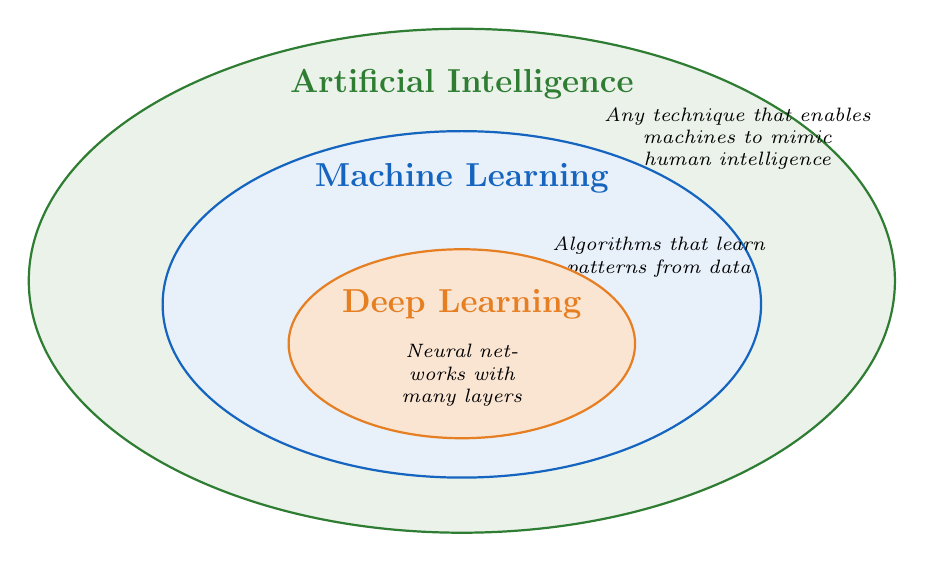
\begin{tikzpicture}[
    every node/.style={font=\small, align=center}
]
% AI circle
\draw[fill=alfaisalgreen!10, draw=alfaisalgreen, thick] (0,0) ellipse (5.5cm and 3.2cm);
\node[font=\large\bfseries, color=alfaisalgreen] at (0, 2.5) {Artificial Intelligence};
\node[font=\scriptsize\itshape, text width=4cm] at (3.5, 1.8) {Any technique that enables\\machines to mimic\\human intelligence};

% ML circle
\draw[fill=questionblue!10, draw=questionblue, thick] (0,-0.3) ellipse (3.8cm and 2.2cm);
\node[font=\large\bfseries, color=questionblue] at (0, 1.3) {Machine Learning};
\node[font=\scriptsize\itshape, text width=3.5cm] at (2.5, 0.3) {Algorithms that learn\\patterns from data};

% DL circle
\draw[fill=warnorange!20, draw=warnorange, thick] (0,-0.8) ellipse (2.2cm and 1.2cm);
\node[font=\large\bfseries, color=warnorange] at (0, -0.3) {Deep Learning};
\node[font=\scriptsize\itshape, text width=2.5cm] at (0, -1.2) {Neural networks with\\many layers};
\end{tikzpicture}
\end{center}

\begin{tcolorbox}[intuitionbox={Key Insight}]
\textbf{AI} is the broadest goal: making machines behave intelligently. \textbf{ML} is one approach: letting machines learn from data instead of being explicitly programmed. \textbf{DL} is one type of ML: using deep neural networks (many layers) that can automatically learn hierarchical features from raw data.
\end{tcolorbox}

\subsection{What Makes Deep Learning ``Deep''?}

A neural network is ``deep'' when it has \textbf{multiple hidden layers} (typically more than two). Each layer learns increasingly abstract representations:
\begin{itemize}[leftmargin=1.5em]
    \item \textbf{Layer 1}: raw signals (edges, pixel intensities)
    \item \textbf{Layer 2}: simple patterns (textures, curves)
    \item \textbf{Layer 3+}: complex concepts (eyes, wheels, sentences)
\end{itemize}

The depth enables the network to compose simple features into complex, high-level representations---this is the power of deep learning.

% ============================================================
% 2. TRADITIONAL PROGRAMMING VS MACHINE LEARNING
% ============================================================
\section{Traditional Programming vs.\ Machine Learning}

\subsection{Two Paradigms}

\begin{center}
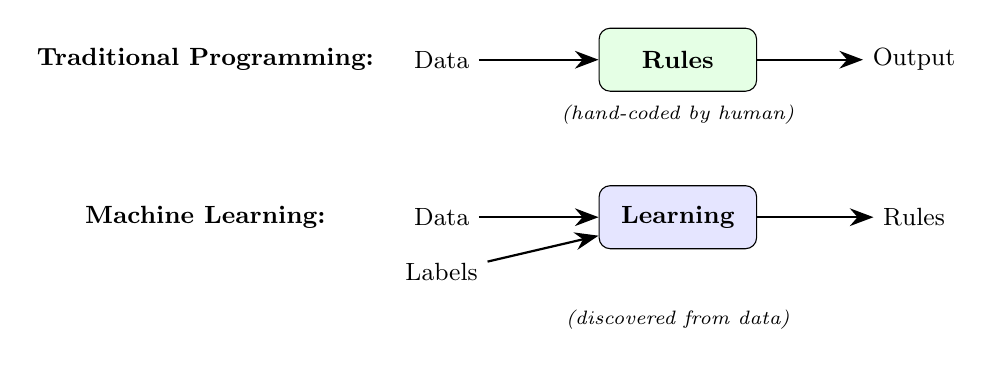
\begin{tikzpicture}[
    box/.style={draw, rounded corners, fill=green!10, minimum height=0.8cm, minimum width=2cm, font=\small\bfseries},
    io/.style={font=\small},
    arr/.style={-{Stealth[length=3mm]}, thick}
]
% Traditional
\node[io, font=\small\bfseries] at (-4, 2) {Traditional Programming:};
\node[io] (td) at (-1, 2) {Data};
\node[box] (tr) at (2, 2) {Rules};
\node[io] (to) at (5, 2) {Output};
\draw[arr] (td) -- (tr);
\draw[arr] (tr) -- (to);
\node[io, font=\scriptsize\itshape] at (2, 1.3) {(hand-coded by human)};

% ML
\node[io, font=\small\bfseries] at (-4, 0) {Machine Learning:};
\node[io] (md) at (-1, 0) {Data};
\node[box, fill=blue!10] (ml) at (2, 0) {Learning};
\node[io] (mo) at (5, 0) {Rules};
\draw[arr] (md) -- (ml);
\draw[arr] (ml) -- (mo);
\node[io] (ml2) at (-1, -0.7) {Labels};
\draw[arr] (ml2) -- (ml);
\node[io, font=\scriptsize\itshape] at (2, -1.3) {(discovered from data)};
\end{tikzpicture}
\end{center}

\begin{tcolorbox}[intuitionbox={Intuition}]
\textbf{Traditional programming}: a human writes explicit rules (``if temperature $>$ 30, turn on AC'').\\
\textbf{Machine learning}: the computer discovers the rules by looking at examples (data + labels). This is essential when the rules are too complex to write by hand---such as recognizing faces, translating languages, or understanding speech.
\end{tcolorbox}

\subsection{When to Use Which?}

\begin{center}
\renewcommand{\arraystretch}{1.3}
\begin{tabular}{@{}lcc@{}}
\toprule
\textbf{Criterion} & \textbf{Traditional} & \textbf{Machine Learning} \\
\midrule
Rules are known and simple & \checkmark & \\
Rules are complex or unknown & & \checkmark \\
Large labeled data available & & \checkmark \\
Interpretability required & \checkmark & \\
Pattern recognition needed & & \checkmark \\
\bottomrule
\end{tabular}
\end{center}

% ============================================================
% 3. DATA CATEGORIES
% ============================================================
\section{Data Categories}

\subsection{Structured vs.\ Unstructured Data}

\begin{center}
\renewcommand{\arraystretch}{1.3}
\begin{tabular}{@{}p{3cm}p{5.5cm}p{5.5cm}@{}}
\toprule
& \textbf{Structured Data} & \textbf{Unstructured Data} \\
\midrule
\textbf{Format} & Tables, rows, columns & No fixed schema \\
\textbf{Examples} & Spreadsheets, SQL databases, CSV files & Images, text, audio, video \\
\textbf{Processing} & Traditional ML works well & Deep learning excels \\
\textbf{Volume} & Typically smaller & $\sim$80\% of all data generated \\
\textbf{Feature extraction} & Features are explicit (columns) & Features must be learned \\
\bottomrule
\end{tabular}
\end{center}

\begin{tcolorbox}[warnbox={Key Point}]
Deep learning's greatest advantage is its ability to process \textbf{unstructured data}---images, text, audio---without requiring manual feature engineering. This is why DL has revolutionized computer vision and NLP, where the input is inherently unstructured.
\end{tcolorbox}

% ============================================================
% 4. SUPERVISED VS UNSUPERVISED LEARNING
% ============================================================
\section{Learning Paradigms}

\subsection{Supervised Learning}

The model learns from \textbf{labeled data}---input-output pairs $(x_i, y_i)$. The goal is to learn a function $f$ such that $f(x) \approx y$.

\begin{itemize}[leftmargin=1.5em]
    \item \textbf{Classification}: output is a discrete category (e.g., spam vs.\ not spam, cat vs.\ dog)
    \item \textbf{Regression}: output is a continuous value (e.g., house price, temperature prediction)
\end{itemize}

\subsection{Unsupervised Learning}

The model learns from \textbf{unlabeled data}---it must discover patterns on its own.

\begin{itemize}[leftmargin=1.5em]
    \item \textbf{Clustering}: grouping similar data points (e.g., customer segmentation)
    \item \textbf{Dimensionality reduction}: compressing data while preserving structure (e.g., PCA, t-SNE)
    \item \textbf{Generative models}: learning the underlying data distribution (e.g., GANs, VAEs)
\end{itemize}

\subsection{Reinforcement Learning}

An \textbf{agent} learns by interacting with an \textbf{environment}, receiving \textbf{rewards} or \textbf{penalties} for its actions. The goal is to learn a \textbf{policy} that maximizes cumulative reward.

\begin{itemize}[leftmargin=1.5em]
    \item Examples: game playing (AlphaGo), robotics, autonomous driving
    \item No labeled data---the agent learns from trial and error
\end{itemize}

\begin{tcolorbox}[questionbox={Self-Check Q1}]
A company wants to automatically organize customer support emails into topics without any predefined categories. Which learning paradigm should they use? Why? \textit{(Solution in Appendix)}
\end{tcolorbox}

% ============================================================
% 5. MACHINE LEARNING VS DEEP LEARNING
% ============================================================
\section{Machine Learning vs.\ Deep Learning}

\subsection{Six Key Differences}

\begin{center}
\renewcommand{\arraystretch}{1.4}
\begin{tabular}{@{}p{3.2cm}p{5.2cm}p{5.2cm}@{}}
\toprule
\textbf{Aspect} & \textbf{Machine Learning} & \textbf{Deep Learning} \\
\midrule
\textbf{Feature extraction} & Manual (human-designed) & Automatic (learned from data) \\
\textbf{Data dependency} & Can work with small datasets & Requires large datasets \\
\textbf{Computation} & CPU is often sufficient & Requires GPU/TPU \\
\textbf{Interpretability} & Interpretable (white box) & Opaque (black box) \\
\textbf{Versatility} & Domain-specific features & Same architecture across domains \\
\textbf{Performance vs.\ data} & Plateaus with more data & Keeps improving with more data \\
\bottomrule
\end{tabular}
\end{center}

\subsection{The Feature Extraction Gap}

This is the most important difference. In traditional ML:

\begin{enumerate}[leftmargin=1.5em]
    \item A domain expert designs features (e.g., ``count the number of edges,'' ``compute the histogram of gradients'')
    \item These features are fed to a classifier (SVM, Random Forest, etc.)
    \item If the features are poor, the model fails---no matter how good the classifier is
\end{enumerate}

In deep learning, the network learns its own features:

\begin{center}
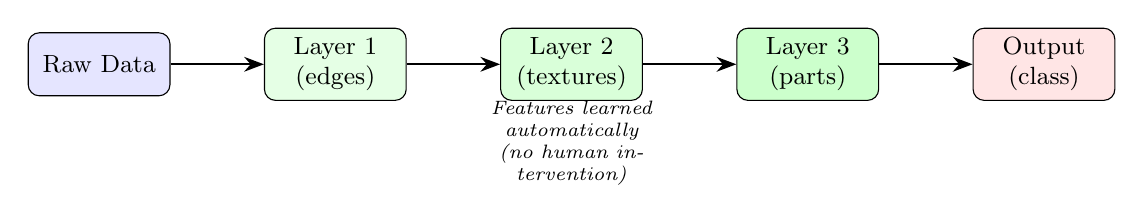
\begin{tikzpicture}[
    box/.style={draw, rounded corners, minimum height=0.8cm, minimum width=1.8cm, font=\small, align=center},
    arr/.style={-{Stealth[length=2.5mm]}, thick}
]
\node[box, fill=blue!10] (raw) at (0,0) {Raw Data};
\node[box, fill=green!10] (l1) at (3,0) {Layer 1\\(edges)};
\node[box, fill=green!15] (l2) at (6,0) {Layer 2\\(textures)};
\node[box, fill=green!20] (l3) at (9,0) {Layer 3\\(parts)};
\node[box, fill=red!10] (out) at (12,0) {Output\\(class)};
\draw[arr] (raw) -- (l1);
\draw[arr] (l1) -- (l2);
\draw[arr] (l2) -- (l3);
\draw[arr] (l3) -- (out);
\node[font=\scriptsize\itshape, text width=3cm, align=center] at (6, -1) {Features learned automatically\\(no human intervention)};
\end{tikzpicture}
\end{center}

\begin{tcolorbox}[intuitionbox={Performance Scaling}]
Traditional ML performance \textbf{plateaus} as data increases---the manually designed features become the bottleneck. Deep learning performance \textbf{keeps improving} with more data because it can learn increasingly rich representations. This is why DL dominates in the era of big data.
\end{tcolorbox}

% ============================================================
% 6. COMPUTER VISION FOUNDATIONS
% ============================================================
\section{Computer Vision Foundations}

\subsection{How Computers See Images}

An image is stored as a \textbf{matrix of numbers}. Each pixel has an intensity value in the range $[0, 255]$:

\begin{itemize}[leftmargin=1.5em]
    \item \textbf{Grayscale image}: a single 2D matrix of size $H \times W$
    \item \textbf{Color image (RGB)}: three 2D matrices stacked---one for Red, one for Green, one for Blue
    \item A color image of size $224 \times 224$ has $224 \times 224 \times 3 = 150{,}528$ values
\end{itemize}

\begin{tcolorbox}[intuitionbox={Intuition}]
When you see a photograph, your brain instantly recognizes objects. A computer sees only a grid of numbers. The challenge of computer vision is: \textbf{how do we go from a matrix of pixel values to semantic understanding} (``this is a cat'')?
\end{tcolorbox}

\subsection{From Pixels to Features}

Traditional computer vision used handcrafted feature descriptors:
\begin{itemize}[leftmargin=1.5em]
    \item \textbf{SIFT} (Scale-Invariant Feature Transform): detects keypoints
    \item \textbf{HOG} (Histogram of Oriented Gradients): captures edge directions
    \item These features were then fed to classifiers like SVMs
\end{itemize}

The problem: designing good features required deep domain expertise and worked only for specific tasks. Deep learning changed this by learning features directly from data.

% ============================================================
% 7. THE IMAGENET CHALLENGE
% ============================================================
\section{The ImageNet Challenge}

\subsection{What is ImageNet?}

ImageNet is a large-scale visual recognition benchmark:
\begin{itemize}[leftmargin=1.5em]
    \item $\sim$1.2 million training images
    \item 1,000 object categories
    \item The \textbf{ImageNet Large Scale Visual Recognition Challenge (ILSVRC)} ran from 2010 to 2017
\end{itemize}

\subsection{The Deep Learning Revolution}

\begin{center}
\renewcommand{\arraystretch}{1.3}
\begin{tabular}{@{}cccp{5cm}@{}}
\toprule
\textbf{Year} & \textbf{Model} & \textbf{Top-5 Error} & \textbf{Significance} \\
\midrule
2010 & NEC-UIUC & 28.2\% & Handcrafted features \\
2012 & \textbf{AlexNet} & \textbf{16.4\%} & First deep CNN to win; started the DL revolution \\
2014 & GoogLeNet & 6.7\% & Inception modules \\
2014 & VGG & 7.3\% & Deeper is better (19 layers) \\
2015 & \textbf{ResNet} & \textbf{3.57\%} & 152 layers; surpassed human-level performance \\
\midrule
--- & Human & 5.1\% & Human-level benchmark \\
\bottomrule
\end{tabular}
\end{center}

\begin{tcolorbox}[warnbox={Turning Point: 2012}]
The \textbf{AlexNet moment} (Krizhevsky et al., 2012) was a watershed event. AlexNet reduced the error rate from 28.2\% to 16.4\%---a \textbf{40\% relative improvement}---using a deep CNN trained on GPUs. This single result convinced the entire AI community that deep learning was viable, and every winner after 2012 used deep neural networks.
\end{tcolorbox}

\begin{tcolorbox}[questionbox={Self-Check Q2}]
In 2015, ResNet achieved a top-5 error of 3.57\%, while human-level performance is approximately 5.1\%. Does this mean ResNet ``sees'' better than humans? What does this comparison really tell us? \textit{(Solution in Appendix)}
\end{tcolorbox}

% ============================================================
% 8. CNNS
% ============================================================
\section{Convolutional Neural Networks (CNNs)}

\subsection{Core Idea}

CNNs exploit the \textbf{spatial structure} of images by using \textbf{local filters} (kernels) that slide across the input, detecting patterns at every spatial position. Key properties:

\begin{itemize}[leftmargin=1.5em]
    \item \textbf{Parameter sharing}: the same filter is applied across the entire image (far fewer parameters than a fully connected network)
    \item \textbf{Local connectivity}: each neuron connects only to a small region of the input
    \item \textbf{Translation invariance}: a cat is a cat regardless of where it appears in the image
\end{itemize}

\subsection{Building Blocks of a CNN}

\subsubsection*{1.\ Convolution Layer}

A filter of size $k \times k$ slides across the input, computing element-wise multiplication and summation at each position:

\begin{equation}
\text{Output}(i,j) = \sum_{m=0}^{k-1} \sum_{n=0}^{k-1} \text{Input}(i+m,\; j+n) \cdot \text{Filter}(m,n) + b
\end{equation}

\textbf{Output size formula:}
\begin{equation}
\boxed{O = \frac{W - K + 2P}{S} + 1}
\end{equation}

where $W$ = input size, $K$ = kernel size, $P$ = padding, $S$ = stride.

\textbf{Example:} Input $32 \times 32$, kernel $5 \times 5$, padding $= 0$, stride $= 1$:
\[
O = \frac{32 - 5 + 0}{1} + 1 = 28
\]

\subsubsection*{2.\ Activation Function (ReLU)}

After each convolution, a non-linearity is applied:
\[
\text{ReLU}(x) = \max(0, x)
\]
This introduces non-linearity, allowing the network to learn complex patterns. Negative values are set to zero.

\subsubsection*{3.\ Pooling Layer}

Reduces the spatial dimensions while retaining the most important information:
\begin{itemize}[leftmargin=1.5em]
    \item \textbf{Max pooling}: takes the maximum value in each window (most common)
    \item \textbf{Average pooling}: takes the mean value in each window
    \item Typical: $2 \times 2$ window with stride 2, reducing each dimension by half
\end{itemize}

\subsubsection*{4.\ Fully Connected (FC) Layer}

After several convolution + pooling stages, the feature maps are \textbf{flattened} into a 1D vector and fed to fully connected layers that perform classification.

\subsection{Feature Learning Hierarchy}

CNNs learn a hierarchy of increasingly abstract features:

\begin{center}
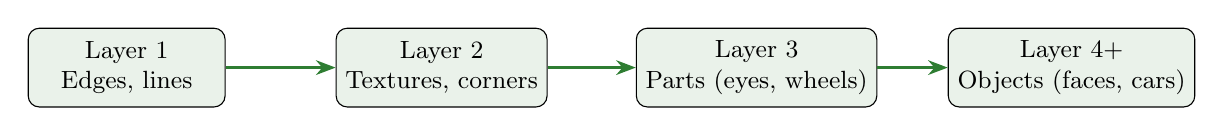
\begin{tikzpicture}[
    box/.style={draw, rounded corners, fill=alfaisalgreen!10, minimum height=1cm, minimum width=2.5cm, font=\small, align=center},
    arr/.style={-{Stealth[length=2.5mm]}, thick, alfaisalgreen}
]
\node[box] (l1) at (0,0) {Layer 1\\Edges, lines};
\node[box] (l2) at (4,0) {Layer 2\\Textures, corners};
\node[box] (l3) at (8,0) {Layer 3\\Parts (eyes, wheels)};
\node[box] (l4) at (12,0) {Layer 4+\\Objects (faces, cars)};
\draw[arr] (l1) -- (l2);
\draw[arr] (l2) -- (l3);
\draw[arr] (l3) -- (l4);
\end{tikzpicture}
\end{center}

\begin{tcolorbox}[intuitionbox={Intuition}]
Think of each layer as asking increasingly sophisticated questions. Layer~1: ``Are there edges here?'' Layer~2: ``Do edges form textures?'' Layer~3: ``Do textures form parts?'' Layer~4: ``Do parts form a recognizable object?'' This compositionality is why deep networks are so powerful.
\end{tcolorbox}

\begin{tcolorbox}[questionbox={Self-Check Q3}]
Given an input image of size $64 \times 64$, a convolution layer with 32 filters of size $3 \times 3$, padding $= 1$, and stride $= 1$, what is the output size? How many learnable parameters does this layer have (including biases)? \textit{(Solution in Appendix)}
\end{tcolorbox}

% ============================================================
% 9. DL EVOLUTION 2010-2015
% ============================================================
\section{Deep Learning Evolution: 2010--2015}

\subsection{From Handcrafted Features to Learned Representations}

\begin{center}
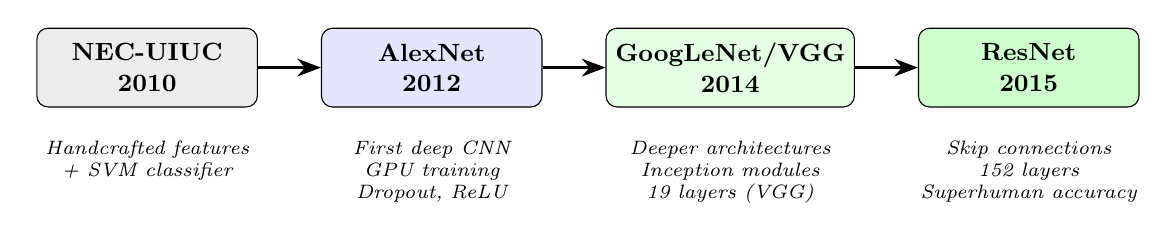
\begin{tikzpicture}[
    node distance=0.8cm,
    box/.style={draw, rounded corners, minimum height=1cm, minimum width=2.8cm, font=\small\bfseries, align=center},
    arr/.style={-{Stealth[length=3mm]}, thick}
]
\node[box, fill=gray!15] (nec) {NEC-UIUC\\2010};
\node[box, fill=blue!10, right=of nec] (alex) {AlexNet\\2012};
\node[box, fill=green!10, right=of alex] (gv) {GoogLeNet/VGG\\2014};
\node[box, fill=green!20, right=of gv] (res) {ResNet\\2015};

\draw[arr] (nec) -- (alex);
\draw[arr] (alex) -- (gv);
\draw[arr] (gv) -- (res);

\node[below=0.3cm, font=\scriptsize\itshape, text width=2.8cm, align=center] at (nec.south) {Handcrafted features\\+ SVM classifier};
\node[below=0.3cm, font=\scriptsize\itshape, text width=2.8cm, align=center] at (alex.south) {First deep CNN\\GPU training\\Dropout, ReLU};
\node[below=0.3cm, font=\scriptsize\itshape, text width=2.8cm, align=center] at (gv.south) {Deeper architectures\\Inception modules\\19 layers (VGG)};
\node[below=0.3cm, font=\scriptsize\itshape, text width=2.8cm, align=center] at (res.south) {Skip connections\\152 layers\\Superhuman accuracy};
\end{tikzpicture}
\end{center}

\textbf{Key innovations at each stage:}
\begin{itemize}[leftmargin=1.5em]
    \item \textbf{AlexNet (2012)}: demonstrated that deep CNNs trained on GPUs with ReLU activation and dropout regularization dramatically outperform handcrafted features
    \item \textbf{VGG (2014)}: showed that using many small ($3\times 3$) filters is better than fewer large filters---deeper is better
    \item \textbf{GoogLeNet (2014)}: introduced Inception modules that apply multiple filter sizes in parallel, capturing multi-scale features efficiently
    \item \textbf{ResNet (2015)}: introduced \textbf{skip (residual) connections} that allow gradients to flow directly through the network, enabling training of extremely deep networks (152 layers)
\end{itemize}

\begin{tcolorbox}[intuitionbox={Why ResNet Works}]
In very deep networks, adding more layers can actually \textbf{hurt} performance (degradation problem). ResNet solves this with skip connections: if a layer has nothing useful to learn, it can simply pass the input through unchanged ($\mathcal{F}(x) + x$). The network only needs to learn the \textbf{residual}---the difference from the identity mapping.
\end{tcolorbox}

% ============================================================
% 10. CV TASKS
% ============================================================
\section{Computer Vision Tasks}

The major computer vision tasks form a hierarchy of increasing complexity:

\begin{center}
\renewcommand{\arraystretch}{1.4}
\begin{tabular}{@{}p{3.5cm}p{4.5cm}p{5cm}@{}}
\toprule
\textbf{Task} & \textbf{Question Answered} & \textbf{Output} \\
\midrule
\textbf{Classification} & ``What is in the image?'' & Single label (e.g., ``cat'') \\
\textbf{Localization} & ``Where is it?'' & Label + bounding box \\
\textbf{Object Detection} & ``Where are all objects?'' & Multiple labels + bounding boxes \\
\textbf{Instance Segmentation} & ``Which exact pixels belong to each object?'' & Pixel-level mask per instance \\
\bottomrule
\end{tabular}
\end{center}

\begin{tcolorbox}[intuitionbox={Intuition}]
Think of it as increasing levels of detail:\\
\textbf{Classification}: ``There's a cat.''\\
\textbf{Localization}: ``There's a cat, and it's in the top-right corner.''\\
\textbf{Detection}: ``There are 2 cats and 1 dog, here's where each one is.''\\
\textbf{Segmentation}: ``Here are the exact pixel boundaries of each animal.''
\end{tcolorbox}

% ============================================================
% 11. GANs
% ============================================================
\section{Generative Adversarial Networks (GANs)}

\subsection{The Core Idea}

A GAN consists of two neural networks competing against each other:

\begin{center}
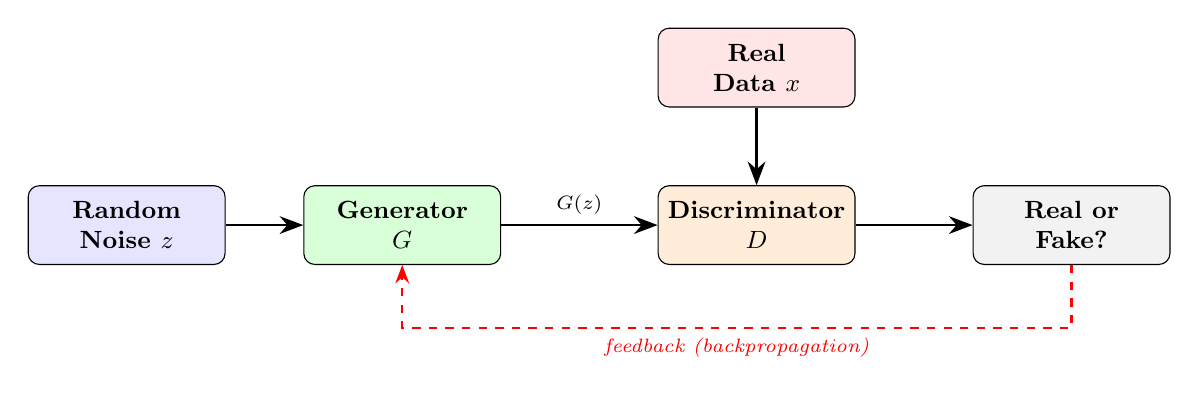
\begin{tikzpicture}[
    box/.style={draw, rounded corners, minimum height=1cm, minimum width=2.5cm, font=\small\bfseries, align=center},
    arr/.style={-{Stealth[length=3mm]}, thick}
]
\node[box, fill=blue!10] (z) at (0,0) {Random\\Noise $z$};
\node[box, fill=green!15] (g) at (3.5,0) {Generator\\$G$};
\node[box, fill=orange!15] (d) at (8,0) {Discriminator\\$D$};
\node[box, fill=gray!10] (out) at (12,0) {Real or\\Fake?};

\node[box, fill=red!10] (real) at (8, 2) {Real\\Data $x$};

\draw[arr] (z) -- (g);
\draw[arr] (g) -- node[above, font=\scriptsize] {$G(z)$} (d);
\draw[arr] (real) -- (d);
\draw[arr] (d) -- (out);

\draw[-{Stealth}, thick, dashed, red] (out.south) -- ++(0,-0.8) -| (g.south) node[pos=0.25, below, font=\scriptsize\itshape] {feedback (backpropagation)};
\end{tikzpicture}
\end{center}

\begin{itemize}[leftmargin=1.5em]
    \item \textbf{Generator} ($G$): takes random noise $z$ and produces fake data $G(z)$. Goal: fool the discriminator.
    \item \textbf{Discriminator} ($D$): takes an input (real or fake) and outputs a probability that it is real. Goal: correctly distinguish real from fake.
\end{itemize}

\begin{tcolorbox}[intuitionbox={The Counterfeiter Analogy}]
The \textbf{Generator} is like a counterfeiter trying to produce fake money. The \textbf{Discriminator} is like a detective trying to catch counterfeit bills. As the detective improves, the counterfeiter must produce better fakes. As the counterfeiter improves, the detective must get better at spotting fakes. Both improve through this adversarial process until the fake money is indistinguishable from real money.
\end{tcolorbox}

\subsection{The GAN Loss Functions}

The GAN training objective is a \textbf{minimax (zero-sum) game}:

\begin{equation}
\boxed{\min_G \max_D\; V(D, G) = \mathbb{E}_{x \sim p_{\text{data}}}[\log D(x)] + \mathbb{E}_{z \sim p_z}[\log(1 - D(G(z)))]}
\end{equation}

Breaking this down into each player's perspective:

\medskip
\noindent\textbf{Discriminator's objective} (maximize):
\begin{equation}
\mathcal{L}_D = \mathbb{E}_{x \sim p_{\text{data}}}[\log D(x)] + \mathbb{E}_{z \sim p_z}[\log(1 - D(G(z)))]
\end{equation}
\begin{itemize}[leftmargin=1.5em]
    \item $\log D(x)$: $D$ wants $D(x) \to 1$ for real data (maximize $\log 1 = 0$)
    \item $\log(1 - D(G(z)))$: $D$ wants $D(G(z)) \to 0$ for fake data (maximize $\log 1 = 0$)
\end{itemize}

\noindent\textbf{Generator's objective} (minimize):
\begin{equation}
\mathcal{L}_G = \mathbb{E}_{z \sim p_z}[\log(1 - D(G(z)))]
\end{equation}
\begin{itemize}[leftmargin=1.5em]
    \item $G$ wants $D(G(z)) \to 1$, so $\log(1 - 1) = \log 0 \to -\infty$ (minimized)
    \item In practice, $G$ maximizes $\log D(G(z))$ instead (better gradient signal early in training)
\end{itemize}

\subsection{Training Process}

GAN training alternates between two steps:
\begin{enumerate}[leftmargin=1.5em]
    \item \textbf{Train $D$}: Fix $G$, update $D$ to better classify real vs.\ fake
    \item \textbf{Train $G$}: Fix $D$, update $G$ to better fool $D$
\end{enumerate}

At equilibrium: $D(x) = 0.5$ for all inputs---the discriminator cannot tell real from fake.

\subsection{Applications}

\begin{itemize}[leftmargin=1.5em]
    \item \textbf{Image synthesis}: generating photorealistic faces (StyleGAN)
    \item \textbf{Image-to-image translation}: converting sketches to photos, day to night
    \item \textbf{Super-resolution}: enhancing low-resolution images
    \item \textbf{Data augmentation}: generating synthetic training data
    \item \textbf{Domain adaptation}: adapting models from one domain (e.g., synthetic data) to another (e.g., real-world data)
\end{itemize}

\begin{tcolorbox}[questionbox={Self-Check Q4}]
In a GAN, what happens if the discriminator becomes too strong too quickly? Why is balancing $G$ and $D$ training important? \textit{(Solution in Appendix)}
\end{tcolorbox}

% ============================================================
% 12. NLP EVOLUTION TIMELINE
% ============================================================
\section{NLP Evolution Timeline}

Natural Language Processing has undergone a series of paradigm shifts:

\begin{center}
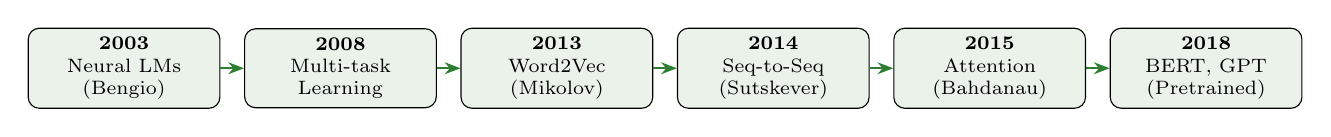
\begin{tikzpicture}[
    node distance=0.3cm,
    evt/.style={draw, rounded corners, fill=alfaisalgreen!10, minimum height=0.7cm, font=\scriptsize, align=center, text width=2.2cm},
    arr/.style={-{Stealth[length=2mm]}, thick, alfaisalgreen}
]
\node[evt] (n1) at (0,0) {\textbf{2003}\\Neural LMs\\(Bengio)};
\node[evt, right=of n1] (n2) {\textbf{2008}\\Multi-task\\Learning};
\node[evt, right=of n2] (n3) {\textbf{2013}\\Word2Vec\\(Mikolov)};
\node[evt, right=of n3] (n4) {\textbf{2014}\\Seq-to-Seq\\(Sutskever)};
\node[evt, right=of n4] (n5) {\textbf{2015}\\Attention\\(Bahdanau)};
\node[evt, right=of n5] (n6) {\textbf{2018}\\BERT, GPT\\(Pretrained)};

\draw[arr] (n1) -- (n2);
\draw[arr] (n2) -- (n3);
\draw[arr] (n3) -- (n4);
\draw[arr] (n4) -- (n5);
\draw[arr] (n5) -- (n6);
\end{tikzpicture}
\end{center}

\begin{itemize}[leftmargin=1.5em]
    \item \textbf{2003 -- Neural Language Models}: Bengio et al.\ proposed learning word representations as part of a language model, replacing n-gram count-based methods
    \item \textbf{2008 -- Multi-task Learning}: showed that a single neural network could learn multiple NLP tasks simultaneously, learning shared representations
    \item \textbf{2013 -- Word2Vec}: Mikolov et al.\ introduced efficient training of word embeddings; demonstrated that word vectors capture semantic relationships (e.g., king $-$ man $+$ woman $\approx$ queen)
    \item \textbf{2014 -- Sequence-to-Sequence}: Sutskever et al.\ introduced encoder-decoder architecture for machine translation, processing entire sentences as sequences
    \item \textbf{2015 -- Attention Mechanism}: Bahdanau et al.\ allowed models to focus on relevant parts of the input, solving the information bottleneck of fixed-length encoding
    \item \textbf{2018 -- Pretrained Models}: BERT (Google) and GPT (OpenAI) showed that pretraining on massive text corpora and fine-tuning on specific tasks achieves state-of-the-art results across NLP
\end{itemize}

\begin{tcolorbox}[warnbox={The Big Shift}]
The evolution from Word2Vec (2013) to BERT/GPT (2018) represents a shift from \textbf{static word embeddings} (same vector for ``bank'' in all contexts) to \textbf{contextual embeddings} (different vector depending on surrounding words). This is the central theme of this course.
\end{tcolorbox}

% ============================================================
% 13. NLP MODELS OVERVIEW
% ============================================================
\section{NLP Models: RNN, LSTM, GRU}

\subsection{Recurrent Neural Networks (RNN)}

RNNs process sequences \textbf{one element at a time}, maintaining a hidden state that serves as memory:

\begin{equation}
h_t = \tanh(W_h \cdot h_{t-1} + W_x \cdot x_t + b)
\end{equation}

\textbf{Strengths}: natural fit for sequential data, parameter sharing across time steps.\\
\textbf{Weakness}: \textbf{vanishing gradient problem}---when sequences are long, gradients shrink exponentially during backpropagation through time, making it nearly impossible to learn long-range dependencies.

\begin{tcolorbox}[intuitionbox={Why Gradients Vanish}]
During backpropagation, the gradient is multiplied by $W_h$ at each time step. If the eigenvalues of $W_h$ are $< 1$, repeated multiplication drives the gradient to zero. For a sequence of length 100: $0.9^{100} \approx 0.00003$.
\end{tcolorbox}

\subsection{Long Short-Term Memory (LSTM)}

LSTM solves the vanishing gradient problem by introducing a \textbf{cell state} $C_t$ and three \textbf{gates}:

\begin{itemize}[leftmargin=1.5em]
    \item \textbf{Forget gate}: $f_t = \sigma(W_f [h_{t-1}, x_t] + b_f)$ --- what to discard
    \item \textbf{Input gate}: $i_t = \sigma(W_i [h_{t-1}, x_t] + b_i)$ --- what to store
    \item \textbf{Output gate}: $o_t = \sigma(W_o [h_{t-1}, x_t] + b_o)$ --- what to output
    \item \textbf{Cell update}: $C_t = f_t \cdot C_{t-1} + i_t \cdot \tilde{C}_t$ (additive update preserves gradients)
\end{itemize}

\subsection{Gated Recurrent Unit (GRU)}

GRU simplifies LSTM by merging the cell state and hidden state, using only two gates:

\begin{itemize}[leftmargin=1.5em]
    \item \textbf{Reset gate}: $r_t = \sigma(W_r [h_{t-1}, x_t] + b_r)$ --- how much past to forget
    \item \textbf{Update gate}: $z_t = \sigma(W_z [h_{t-1}, x_t] + b_z)$ --- keep old vs.\ use new
    \item \textbf{Hidden state}: $h_t = (1 - z_t) \cdot h_{t-1} + z_t \cdot \tilde{h}_t$ (interpolation)
\end{itemize}

GRU has fewer parameters, trains faster, and performs comparably to LSTM on many tasks.

% ============================================================
% 14. NLP APPLICATIONS
% ============================================================
\section{NLP Applications}

Deep learning has enabled breakthroughs across a wide range of NLP tasks:

\begin{center}
\renewcommand{\arraystretch}{1.3}
\begin{tabular}{@{}p{4cm}p{5cm}p{4.5cm}@{}}
\toprule
\textbf{Application} & \textbf{Description} & \textbf{Example} \\
\midrule
Text Classification & Assign categories to text & Spam detection, sentiment analysis \\
Information Extraction & Extract structured data from text & Named Entity Recognition (NER) \\
Conversational Agents & Generate contextual responses & Chatbots, virtual assistants \\
Information Retrieval & Find relevant documents & Search engines \\
Question Answering & Answer questions from context & SQuAD, reading comprehension \\
Machine Translation & Translate between languages & Google Translate \\
Text Summarization & Compress text to key points & News summaries \\
\bottomrule
\end{tabular}
\end{center}

\begin{tcolorbox}[intuitionbox={Industry Impact}]
NLP is transforming industries: healthcare (clinical note analysis), finance (sentiment-driven trading), legal (contract analysis), customer service (automated support), and education (automated grading). The common thread is that these applications require understanding \textbf{unstructured text data}, which is where deep learning excels.
\end{tcolorbox}

\begin{tcolorbox}[questionbox={Self-Check Q5}]
A hospital wants to automatically extract drug names, dosages, and conditions from doctors' handwritten clinical notes (after OCR). Which NLP task is this? Which learning paradigm (supervised, unsupervised, or reinforcement) would you use? \textit{(Solution in Appendix)}
\end{tcolorbox}

% ============================================================
% 15. SELF-ATTENTION AND TRANSFORMERS PREVIEW
% ============================================================
\section{Self-Attention and Transformers Preview}

\subsection{The Limitation of RNNs}

RNNs process tokens \textbf{sequentially}: token $t$ must wait for tokens $1, 2, \ldots, t{-}1$ to be processed. This creates two problems:
\begin{enumerate}[leftmargin=1.5em]
    \item \textbf{No parallelization}: training is slow because computations cannot be distributed across GPU cores
    \item \textbf{Information bottleneck}: the entire input sequence is compressed into a single fixed-size vector $h_T$
\end{enumerate}

\subsection{The Self-Attention Innovation}

Self-attention allows every token to \textbf{directly attend to every other token} in the sequence, regardless of distance:

\begin{equation}
\text{Attention}(Q, K, V) = \text{softmax}\!\left(\frac{QK^T}{\sqrt{d_k}}\right) V
\end{equation}

where $Q$ (queries), $K$ (keys), and $V$ (values) are linear projections of the input. The key properties:

\begin{itemize}[leftmargin=1.5em]
    \item \textbf{Parallel computation}: all attention weights are computed simultaneously via matrix multiplication
    \item \textbf{Direct long-range connections}: token 1 can directly attend to token 100 (no gradient chain)
    \item \textbf{Learned relevance}: the model learns which tokens are most relevant to each other through attention weights
\end{itemize}

\subsection{Transformer Architecture (Preview)}

The Transformer (Vaswani et al., 2017) uses self-attention as its core mechanism:

\begin{center}
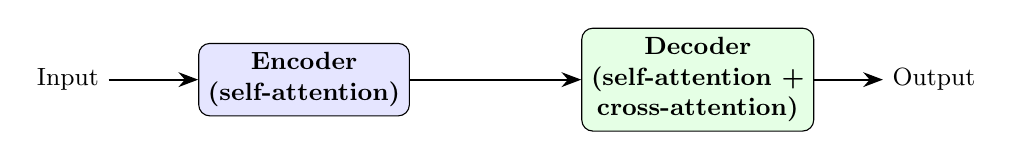
\begin{tikzpicture}[
    box/.style={draw, rounded corners, minimum height=0.8cm, minimum width=2.5cm, font=\small\bfseries, align=center},
    arr/.style={-{Stealth[length=2.5mm]}, thick}
]
\node[box, fill=blue!10] (enc) at (0,0) {Encoder\\(self-attention)};
\node[box, fill=green!10] (dec) at (5,0) {Decoder\\(self-attention +\\cross-attention)};
\node[font=\small] (in) at (-3,0) {Input};
\node[font=\small] (out) at (8,0) {Output};
\draw[arr] (in) -- (enc);
\draw[arr] (enc) -- (dec);
\draw[arr] (dec) -- (out);
\end{tikzpicture}
\end{center}

\begin{itemize}[leftmargin=1.5em]
    \item \textbf{Encoder}: processes the input sequence, producing contextual representations
    \item \textbf{Decoder}: generates the output sequence, attending to both its own previous outputs and the encoder's representations
    \item Both use \textbf{multi-head attention}: multiple attention operations in parallel, each learning different aspects of the relationships between tokens
\end{itemize}

Transformers will be covered in depth in later lectures.

\begin{tcolorbox}[questionbox={Self-Check Q6}]
Why is the scaling factor $\sqrt{d_k}$ needed in the attention formula? What would happen without it? \textit{(Solution in Appendix)}
\end{tcolorbox}

% ============================================================
% 16. SEQUENTIAL DATA AND MODELS
% ============================================================
\section{Sequential Data and Model Architectures}

\subsection{Types of Sequential Data}

Sequential data appears in many domains:
\begin{itemize}[leftmargin=1.5em]
    \item \textbf{Text}: sequences of words or characters
    \item \textbf{Speech}: sequences of audio frames
    \item \textbf{Time series}: stock prices, sensor readings, weather data
    \item \textbf{Video}: sequences of image frames
    \item \textbf{DNA}: sequences of nucleotides (A, C, G, T)
\end{itemize}

\subsection{Sequence-to-Sequence Architectures}

Different tasks require different input-output configurations:

\begin{center}
\renewcommand{\arraystretch}{1.4}
\begin{tabular}{@{}p{3.5cm}p{3.5cm}p{3cm}p{3cm}@{}}
\toprule
\textbf{Architecture} & \textbf{Input $\to$ Output} & \textbf{Example Task} & \textbf{Concrete Example} \\
\midrule
\textbf{One-to-One} & Fixed $\to$ Fixed & Image classification & Image $\to$ ``cat'' \\
\textbf{One-to-Many} & Fixed $\to$ Sequence & Image captioning & Image $\to$ ``A cat sitting on a mat'' \\
\textbf{Many-to-One} & Sequence $\to$ Fixed & Sentiment analysis & ``I love this movie'' $\to$ Positive \\
\textbf{Many-to-Many} (equal) & Sequence $\to$ Sequence & Named entity recognition & Word-by-word tagging \\
\textbf{Many-to-Many} (unequal) & Sequence $\to$ Sequence & Machine translation & English sentence $\to$ Arabic sentence \\
\bottomrule
\end{tabular}
\end{center}

\begin{tcolorbox}[intuitionbox={Intuition}]
The flexibility of sequence models is what makes them so powerful. The \textbf{same underlying architecture} (RNN/LSTM/Transformer) can be configured for any of these patterns simply by changing what you feed in and what you read out.
\end{tcolorbox}

% ============================================================
% 17. ORIGIN OF RNN
% ============================================================
\section{Origin of Recurrent Neural Networks}

\subsection{Elman 1990: ``Finding Structure in Time''}

The concept of recurrent neural networks was introduced by \textbf{Jeffrey Elman} in his seminal 1990 paper \textit{``Finding Structure in Time.''}

\textbf{Key ideas:}
\begin{itemize}[leftmargin=1.5em]
    \item Traditional neural networks treat inputs as independent---they have no notion of \textbf{temporal order}
    \item Elman proposed adding a \textbf{context layer} (hidden state) that stores information from previous time steps
    \item At each time step, the network receives both the current input \textbf{and} a copy of its own previous hidden state
    \item This recurrence gives the network \textbf{memory}---the ability to process sequences where order matters
\end{itemize}

\textbf{The Elman Network:}
\begin{equation}
h_t = f(W_x \cdot x_t + W_h \cdot h_{t-1})
\end{equation}

This is the same equation used in modern RNNs. The context units act as a \textbf{short-term memory}, allowing the network to learn temporal patterns.

\begin{tcolorbox}[warnbox={Historical Significance}]
Elman's 1990 paper demonstrated that simple recurrent networks could learn grammatical structure from sequences of words without being explicitly taught grammar rules. This was a foundational insight: \textbf{structure in language can emerge from processing sequences with memory}. This idea directly led to the RNN, LSTM, GRU, and ultimately the Transformer architectures used today.
\end{tcolorbox}

\begin{tcolorbox}[questionbox={Self-Check Q7}]
Elman's 1990 network and a modern vanilla RNN use essentially the same equation. What key advances between 1990 and 2012 made RNNs practical for real-world applications? Name at least three. \textit{(Solution in Appendix)}
\end{tcolorbox}

% ============================================================
% APPENDIX
% ============================================================
\newpage
\section*{Appendix: Solutions to Self-Check Questions}
\addcontentsline{toc}{section}{Appendix: Solutions to Self-Check Questions}

\subsection*{Q1: Which learning paradigm for organizing emails without predefined categories?}

\textbf{Unsupervised learning}, specifically \textbf{clustering}. Since there are no predefined categories, we cannot use supervised learning (which requires labeled data). Clustering algorithms (e.g., k-means, hierarchical clustering, or topic modeling with LDA) can automatically discover groups of similar emails based on their content. The company can then inspect each cluster to assign meaningful topic labels after the fact. If the company later wants to classify new emails into the discovered categories, they can switch to supervised learning using the clusters as training labels.

\subsection*{Q2: Does ResNet ``see'' better than humans?}

\textbf{Not exactly.} The comparison is misleading for several reasons:

\begin{itemize}[leftmargin=1.5em]
    \item The 5.1\% human error rate was measured on a specific person (Andrej Karpathy) classifying ImageNet images into 1,000 fine-grained categories---many of which are extremely similar dog breeds that require expert knowledge
    \item ResNet excels at this \textbf{narrow task} (classifying among 1,000 specific categories with clean, centered images)
    \item Humans vastly outperform ResNet in: understanding context, recognizing objects in unusual orientations, generalizing from few examples, handling adversarial perturbations, and performing open-ended visual reasoning
    \item The comparison tells us that deep learning has \textbf{surpassed human-level on a specific benchmark}, not that it has achieved general visual intelligence
\end{itemize}

\subsection*{Q3: CNN output size and parameter count}

\textbf{Output spatial size:}
\[
O = \frac{W - K + 2P}{S} + 1 = \frac{64 - 3 + 2(1)}{1} + 1 = 64
\]
With 32 filters, the output is $64 \times 64 \times 32$.

\textbf{Learnable parameters:} Each filter has size $3 \times 3$ and operates on the input (assuming 3 RGB channels): $3 \times 3 \times 3 = 27$ weights per filter, plus 1 bias $= 28$ parameters per filter. With 32 filters: $32 \times 28 = \mathbf{896}$ parameters.

Note: if the input has only 1 channel (grayscale), the count would be $32 \times (3 \times 3 \times 1 + 1) = 320$.

\subsection*{Q4: What if the discriminator becomes too strong?}

If the discriminator becomes too strong too quickly, it will correctly reject all generated samples with high confidence ($D(G(z)) \approx 0$). This causes the generator's gradient to \textbf{vanish}:

\begin{itemize}[leftmargin=1.5em]
    \item The generator's loss involves $\log(1 - D(G(z)))$. When $D(G(z)) \approx 0$, this becomes $\log(1) = 0$, providing \textbf{no useful gradient signal} for the generator to improve
    \item The generator cannot learn because it receives no information about \textit{how} to improve its outputs
    \item This leads to \textbf{mode collapse}: the generator produces limited, repetitive outputs
\end{itemize}

Balancing is crucial because both networks must improve at roughly the same pace. In practice, the discriminator is often trained for fewer steps per iteration, or techniques like label smoothing and gradient penalty are used to prevent it from becoming too confident.

\subsection*{Q5: NLP task for extracting medical information}

This is \textbf{Information Extraction}, specifically \textbf{Named Entity Recognition (NER)}. The task involves identifying and classifying specific entities in text:

\begin{itemize}[leftmargin=1.5em]
    \item Drug names $\to$ DRUG entity
    \item Dosages $\to$ DOSAGE entity
    \item Medical conditions $\to$ CONDITION entity
\end{itemize}

This requires \textbf{supervised learning}: we need a labeled training dataset where medical professionals have annotated clinical notes with the correct entity types. The model (typically a BiLSTM-CRF or fine-tuned BERT) learns to predict entity labels for each token. This is a \textbf{many-to-many} sequence labeling task.

\subsection*{Q6: Why scale by $\sqrt{d_k}$ in attention?}

The dot product $QK^T$ computes the sum of $d_k$ products. As $d_k$ grows, the magnitude of the dot products grows proportionally (assuming unit-variance inputs, the variance of the dot product is $d_k$). Large dot product values push the softmax function into regions with \textbf{extremely small gradients} (saturation):

\begin{itemize}[leftmargin=1.5em]
    \item If $d_k = 512$, dot products can be in the range $[-30, +30]$
    \item $\text{softmax}([30, -30]) \approx [1.0, 0.0]$---essentially a hard, one-hot distribution
    \item Gradients of softmax at saturation are near zero, causing \textbf{vanishing gradients}
\end{itemize}

Dividing by $\sqrt{d_k}$ normalizes the dot products to have unit variance regardless of $d_k$, keeping them in a range where softmax produces \textbf{smooth probability distributions} with healthy gradients.

\subsection*{Q7: What advances made RNNs practical between 1990 and 2012?}

\begin{enumerate}[leftmargin=1.5em]
    \item \textbf{LSTM (Hochreiter \& Schmidhuber, 1997)}: solved the vanishing gradient problem that made vanilla RNNs unable to learn long-range dependencies---this was the most critical theoretical advance
    \item \textbf{GPU computing}: massively parallel hardware (especially NVIDIA GPUs with CUDA) made training large networks on large datasets feasible. Training that took weeks on CPUs could be done in hours on GPUs
    \item \textbf{Large datasets}: the internet enabled collection of massive text and speech corpora needed for training data-hungry deep models
    \item \textbf{Better optimization}: advances in optimization algorithms (Adam, RMSProp), initialization strategies (Xavier/He initialization), and regularization techniques (dropout, batch normalization) made training deep networks more stable
    \item \textbf{Software frameworks}: libraries like Theano (2010), later TensorFlow (2015) and PyTorch (2016), made it dramatically easier to implement, train, and debug neural networks with automatic differentiation
\end{enumerate}

\end{document}
